\subsubsection{Reproducing rheology of Morency and Doin, 2004}
\label{sec:cookbooks-morency-doin}
\textit{This section was contributed by Jonathan Perry-Houts}

Modeling interactions between the upper mantle and the lithosphere can be difficult because
of the dynamic range of temperatures and pressures involved. Many simple material models
will assign very high viscosities at low temperature thermal boundary layers. The
pseudo-brittle rheology described in \cite{MD04} was developed to limit the strength of
lithosphere at low temperature. The effective viscosity can be described as the harmonic mean
of two non-Newtonian rheologies:
\[v_{\text{eff}} = \left(\frac{1}{v_{\text{eff}}^v}+\frac{1}{v_{\text{eff}}^p}\right)^{-1}\]
where
\begin{align*}
  v_{\text{eff}}^v = B \left(\frac{\dot{\epsilon}}{\dot{\epsilon}_\text{ref}}\right)^{-1+1/n_v}
  \exp\left(\frac{E_a +V_a \rho_m g z}{n_v R T}\right),
  \\
  v_{\text{eff}}^p = (\tau_0 + \gamma \rho_m g z) \left( \frac{\dot{\epsilon}^{-1+1/n_p}}
  {\dot{\epsilon}_\text{ref}^{1/n_p}} \right),
\end{align*}
where $B$ is a scaling constant; $\dot{\epsilon}$ is defined as the quadratic sum of the
second invariant of the strain rate tensor and a minimum strain rate, $\dot{\epsilon}_0$;
$\dot{\epsilon}_\text{ref}$ is a reference strain rate; $n_v$, and $n_p$ are stress exponents;
$E_a$ is the activation energy; $V_a$ is the activation volume; $\rho_m$ is the mantle density;
$R$ is the gas constant; $T$ is temperature; $\tau_0$ is the cohesive strength of rocks at
the surface; $\gamma$ is a coefficient of yield stress increase with depth; and $z$ is depth.

By limiting the strength of the lithosphere at low temperature, this rheology allows one to
more realistically model processes like lithospheric delamination and foundering in the
presence of weak crustal layers. A similar model setup to the one described in \cite{MD04}
can be reproduced with the files in the directory \url{cookbooks/morency_doin_2004}.
In particular, the following sections of the input file are important to reproduce the setup:

\note{\cite{MD04} defines the second invariant of the strain rate in a nonstandard way.
    The formulation in the paper is given as $\epsilon_{II} = \sqrt{\frac{1}{2}
    (\epsilon_{11}^2 + \epsilon_{12}^2)}$, where $\epsilon$ is the strain rate tensor.
    For consistency, that is also the formulation implemented in \aspect{}. Because of this
    irregularity it is inadvisable to use this material model for purposes beyond
    reproducing published results.}

\note{The viscosity profile in Figure 1 of \cite{MD04} appears to be wrong. The published
    parameters do not reproduce those viscosities; it is unclear why. The values used here
    get very close. See Figure~\ref{fig:md-1} for an approximate reproduction of the
    original figure.}

\lstinputlisting[language=prmfile]{cookbooks/morency_doin_2004/doc/morency_doin.part.prm.out}

\begin{figure}[h!]
  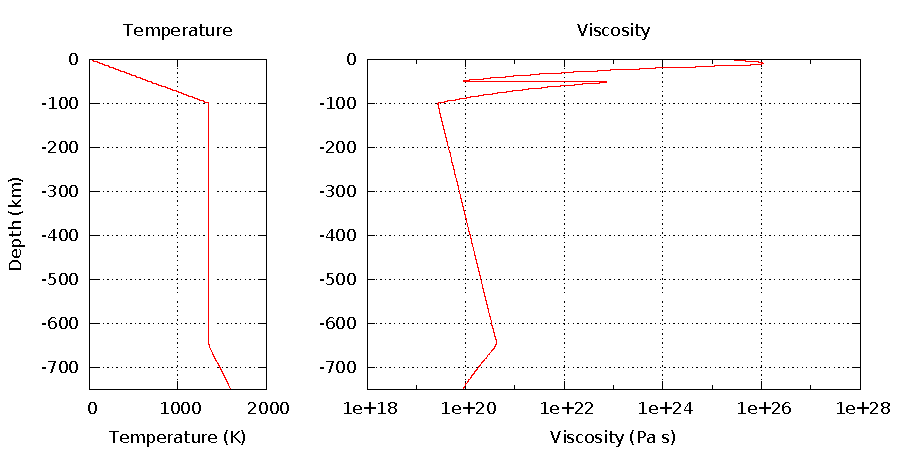
\includegraphics[width=\textwidth]{cookbooks/morency_doin_2004/doc/morency_doin_2004_fig1.pdf}
  \caption{\it Approximate reproduction of figure 1 from \cite{MD04} using the `morency doin'
  material model with almost all default parameters. Note the low-viscosity Moho, enabled by
  the low activation energy of the crustal component.}
  \label{fig:md-1}
\end{figure}

